\documentclass{article}

\usepackage{extramarks}

\usepackage{amsmath}
\usepackage{amsthm}
\usepackage{amssymb}
\usepackage{amsfonts}
\usepackage{caption}
\usepackage{subcaption}
\usepackage{listings}

\usepackage{hyperref}

\usepackage{tikz}

\usepackage{algorithm}
\usepackage{algorithmic}
\usepackage[shortlabels]{enumitem}

\usepackage{float,graphicx}

\usepackage{pgfplots}

\usepackage{adjustbox}


\usepackage{array}
\usepackage{pgfgantt}

\usepackage[utf8]{inputenc}

\usepackage{fancyhdr}
\usepackage{fancybox}



\topmargin=-0.45in
\evensidemargin=0in
\oddsidemargin=0in
\textwidth=6.5in
\textheight=9.0in
\headsep=0.25in

% Listings' Styles

\definecolor{codegreen}{rgb}{0,0.6,0}
\definecolor{codegray}{rgb}{0.5,0.5,0.5}
\definecolor{codepurple}{rgb}{0.58,0,0.82}
\definecolor{backcolour}{rgb}{0.96,0.96,0.96}


\lstdefinestyle{python}{
    backgroundcolor=\color{backcolour},
    commentstyle=\color{codegreen},
    keywordstyle=\color{magenta},
    numberstyle=\tiny\color{codegray},
    stringstyle=\color{codepurple},
    basicstyle=\footnotesize,
    breakatwhitespace=false,
    breaklines=true,
    captionpos=b,
    keepspaces=true,
    numbers=left,
    numbersep=5pt,
    showspaces=false,
    showstringspaces=false,
    showtabs=false,
    tabsize=2
}

\lstset{style=python}
\lstset{language=Python}

\linespread{1.1}
\captionsetup[table]{position=bottom}

\pagestyle{fancy}
\lhead{\groupName}
\chead{\hmwkClass: \hmwkTitle}
\rhead{\today}
\lfoot{\lastxmark}
\cfoot{\thepage}

\renewcommand\headrulewidth{0.4pt}
\renewcommand\footrulewidth{0.4pt}
\renewcommand\qedsymbol{$\blacksquare$}

\setlength\parindent{0pt}

\newcommand{\hmwkTitle}{Assignment Sheet\ \#\hmwkNumber}
\newcommand{\hmwkDueDate}{April 26, 2022}
\newcommand{\hmwkClass}{Machine Learning}
\newcommand{\hmwkAuthorName}{Henri Sota, Enis Mustafaj}
\newcommand{\groupName}{\textbf{Group HB}}

% Homework Number Variable
\newcommand{\hmwkNumber}{10}

%
% Create Problem Sections
%

\newcommand{\enterProblemHeader}[1]{
    \nobreak{}
}

\newcommand{\exitProblemHeader}[1]{
    \stepcounter{#1}
}

\setcounter{secnumdepth}{0}
\newcounter{partCounter}
\newcounter{homeworkProblemCounter}

\setcounter{homeworkProblemCounter}{1}
\nobreak\extramarks{Problem \hmwkNumber \arabic{homeworkProblemCounter}}{}\nobreak{}

%
% Homework Problem Environment
%
% This environment takes an optional argument. When given, it will adjust the
% problem counter. This is useful for when the problems given for your
% assignment aren't sequential. See the last 3 problems of this template for an
% example.
%
\newenvironment{homeworkProblem}[1][-1]{
    \ifnum#1>0
        \setcounter{homeworkProblemCounter}{\hmwkNumber.#1}
    \fi
    \section{Problem \hmwkNumber.\arabic{homeworkProblemCounter}}
    \setcounter{partCounter}{1}
    \enterProblemHeader{homeworkProblemCounter}
}{
    \exitProblemHeader{homeworkProblemCounter}
}


\newcounter{programmingPartCounter}
\newcounter{programmingProblemCounter}

\setcounter{programmingProblemCounter}{1}
\nobreak\extramarks{Programming Problem \hmwkNumber \arabic{programmingProblemCounter}}{}\nobreak{}

%
% Programming Problem Environment
%
% This environment takes an optional argument. When given, it will adjust the
% problem counter. This is useful for when the problems given for your
% assignment aren't sequential. See the last 3 problems of this template for an
% example.
%
\newenvironment{programmingProblem}[1][-1]{
    \ifnum#1>0
        \setcounter{programmingProblemCounter}{\hmwkNumber.#1}
    \fi
    \section{Programming Problem \hmwkNumber.\arabic{programmingProblemCounter}}
    \setcounter{programmingPartCounter}{1}
    \enterProblemHeader{programmingProblemCounter}
}{
    \exitProblemHeader{programmingProblemCounter}
}

\title{
    \vspace{2in}
    \textmd{\textbf{\hmwkClass:\\ \hmwkTitle}}\\
    \normalsize\vspace{0.1in}\small{Due\ on\ \hmwkDueDate\ at 10:00}\\
    \vspace{3in}
}

\author{\groupName \\ \hmwkAuthorName}
\date{}

\renewcommand{\part}[1]{\textbf{\large Part \Alph{partCounter}}\stepcounter{partCounter}\\}

% Useful for algorithms
\newcommand{\alg}[1]{\textsc{\bfseries \footnotesize #1}}

% Alias for the Solution section header
\newcommand{\solution}{\textbf{\large Solution}}
\newcommand{\comment}[1]{} % Multi-line comment

\DeclareMathOperator*{\argmax}{arg\,max}
\DeclareMathOperator*{\argmin}{arg\,min}

\newcommand{\norm}[1]{\left\lVert#1\right\rVert}

\begin{document}
\maketitle
\pagebreak
\begin{homeworkProblem}
In this task, you carry out $K$-means clustering with $K = 3$ by paper and pencil. To this end, you are given the following data
\begin{table}[h!]
    \centering
    \begin{tabular}{c|c|c}
    $i$ & $x_{i}$ & $C^{(0)}(i)$ \\ \hline
    1 & $(15, 7)^{\top}$ & 2 \\
    2 & $(0, -9)^{\top}$ & 1 \\
    3 & $(-2, -5)^{\top}$ & 1 \\
    4 & $(2, 3)^{\top}$ & 0 \\
    5 & $(3, 7)^{\top}$ & 2 \\
    6 & $(18, 12)^{\top}$ & 0
    \end{tabular}
\end{table}

with its initial cluster assignment. Let the clustering algorithm "run" until it finalized its assignment. Finally, draw the just computed clusters in a two-dimensional scatter plot.\\

Recalling Algorithm 14, $K$-means clustering:

\textbf{Input:} input data $\{ (\boldsymbol x_{i}) \}_{i = 1}^{N} (\boldsymbol x_{i} \in \mathbb{R}^{D})$, cluster count $K$\\
\textbf{Output:} cluster assignment $C^{*}$, centroids $\{ \bar{\boldsymbol x}_{k}^{*} \}_{k = 1}^{K}$
\begin{enumerate}
    \item choose initial guess $C^{(0)}$
    \item $s \gets 0$
    \item repeat:
    \begin{enumerate}[a)]
        \item $s \gets s + 1$
        \item $N_{k} \gets |\{ i | C^{(s - 1)}(i) = k \}|$, \quad $k = 1, \ldots, K$
        \item $\boldsymbol m_{k}^{(s)} \gets \frac{1}{N_{k}} \sum_{C^{(s - 1)} (i) = k} \boldsymbol x_{i}, \quad k = 1, \ldots, K$ \quad \textit{(compute centroids)}
        \item $C^{(s)}(i) \gets \text{arg min}_{1 \leq k \leq K} \norm{ \boldsymbol x_{i} - \boldsymbol m_{k}^{(s)} }^{2}, \quad i = 1, \ldots, N$ \quad \textit{(cluster samples around closest centroid)}
    \end{enumerate}
    until $C^{(s)} = C^{(s - 1)}$
    \item $\bar{\boldsymbol x}_{k}^{*} \gets \frac{1}{|\{ i | C^{(s - 1)}(i) = k \}|} \sum_{C^{(s)} (i) = k} \boldsymbol x_{i}, \quad k = 1, \ldots, K$ \quad \textit{(compute final centroids)}
    \item return $C^{*}, \{ \bar{\boldsymbol x}_{k}^{*} \}_{k = 1}^{K}$
\end{enumerate}

With the initial cluster assignment given, we start iterating:\\
\textbf{Iteration 1:}
\begin{enumerate}[a)]
    \item $s \gets s + 1 = 1$
    \item Cluster sizes with the data points based on index: $N_{1} = 2 (\{ 4, 6 \}), N_{2} = 2 (\{ 2, 3 \}), N_{3} = 2 (\{ 1, 5 \})$
    \item Calculating centroids for each cluster:
    \begin{itemize}
        \item $\boldsymbol m_{1}^{(1)} = \frac{1}{2} ((2, 3)^{\top} + (18, 12)^{\top}) = (10, 7.5)^{\top}$
        \item $\boldsymbol m_{2}^{(1)} = \frac{1}{2} ((0, -9)^{\top} + (-2, -5)^{\top}) = (-1, -7)^{\top}$
        \item $\boldsymbol m_{3}^{(1)} = \frac{1}{2} ((15, 7)^{\top} + (3, 7)^{\top}) = (9, 7)^{\top}$
    \end{itemize}
    \item Cluster the samples based on the closest centroid:
    \begin{itemize}
        \item $C^{(1)}(1) = \text{arg min}_{1 \leq k \leq K} \{ 5.02493781, 21.26029163, 6 \}$ = 0
        \item $C^{(1)}(2) = \text{arg min}_{1 \leq k \leq K} \{ 19.29378138, 2.23606798, 18.35755975 \}$ = 1
        \item $C^{(1)}(3) = \text{arg min}_{1 \leq k \leq K} \{ 17.32772345, 2.23606798, 16.2788206 \}$ = 1
        \item $C^{(1)}(4) = \text{arg min}_{1 \leq k \leq K} \{ 9.17877988, 10.44030651, 8.06225775 \}$ = 2
        \item $C^{(1)}(5) = \text{arg min}_{1 \leq k \leq K} \{ 7.01783442, 14.56021978, 6 \}$ = 2
        \item $C^{(1)}(6) = \text{arg min}_{1 \leq k \leq K} \{ 9.17877988, 26.87005769, 10.29563014 \}$ = 0
    \end{itemize}
\end{enumerate}
$C^{1}$ is not the same as $C^{0}$. Continue iteration.\\
\textbf{Iteration 2:}
\begin{enumerate}[a)]
    \item $s \gets s + 1 = 2$
    \item Cluster sizes with the data points based on index: $N_{1} = 2 (\{ 1, 6 \}), N_{2} = 2 (\{ 2, 3 \}), N_{3} = 2 (\{ 4, 5 \})$
    \item Calculating centroids for each cluster:
    \begin{itemize}
        \item $\boldsymbol m_{1}^{(2)} = \frac{1}{2} ((15, 7)^{\top} + (18, 12)^{\top}) = (16.5, 9.5)^{\top}$
        \item $\boldsymbol m_{2}^{(2)} = \frac{1}{2} ((0, -9)^{\top} + (-2, -5)^{\top}) = (-1, -7)^{\top}$
        \item $\boldsymbol m_{3}^{(2)} = \frac{1}{2} ((2, 3)^{\top} + (3, 7)^{\top}) = (2.5, 5)^{\top}$
    \end{itemize}
    \item Cluster the samples based on the closest centroid:
    \begin{itemize}
        \item $C^{(2)}(1) = \text{arg min}_{1 \leq k \leq K} \{ 2.91547595, 21.26029163, 12.658988 \}$ = 0
        \item $C^{(2)}(2) = \text{arg min}_{1 \leq k \leq K} \{ 24.78911051, 2.23606798, 14.22146265 \}$ = 1
        \item $C^{(2)}(3) = \text{arg min}_{1 \leq k \leq K} \{ 23.50531855, 2.23606798, 10.9658561 \}$ = 1
        \item $C^{(2)}(4) = \text{arg min}_{1 \leq k \leq K} \{ 15.89024858, 10.44030651, 2.06155281 \}$ = 2
        \item $C^{(2)}(5) = \text{arg min}_{1 \leq k \leq K} \{ 13.72953022, 14.56021978, 2.06155281 \}$ = 2
        \item $C^{(2)}(6) = \text{arg min}_{1 \leq k \leq K} \{ 2.91547595, 26.87005769, 17.00735135 \}$ = 0
    \end{itemize}
\end{enumerate}
$C^{2}$ is the same as $C^{1}$. Stop iteration.\\

Calculating the final centroids:
\begin{itemize}
    \item $\bar{\boldsymbol x}_{1}^{*} = \frac{1}{2} ((15, 7)^{\top} + (18, 12)^{\top}) = (16.5, 9.5)^{\top}$
    \item $\bar{\boldsymbol x}_{2}^{*} = \frac{1}{2} ((0, -9)^{\top} + (-2, -5)^{\top}) = (-1, -7)^{\top}$
    \item $\bar{\boldsymbol x}_{3}^{*} = \frac{1}{2} ((2, 3)^{\top} + (3, 7)^{\top}) = (2.5, 5)^{\top}$
\end{itemize}

The computed clusters can be seen on the scatter plot below.

\begin{center}
    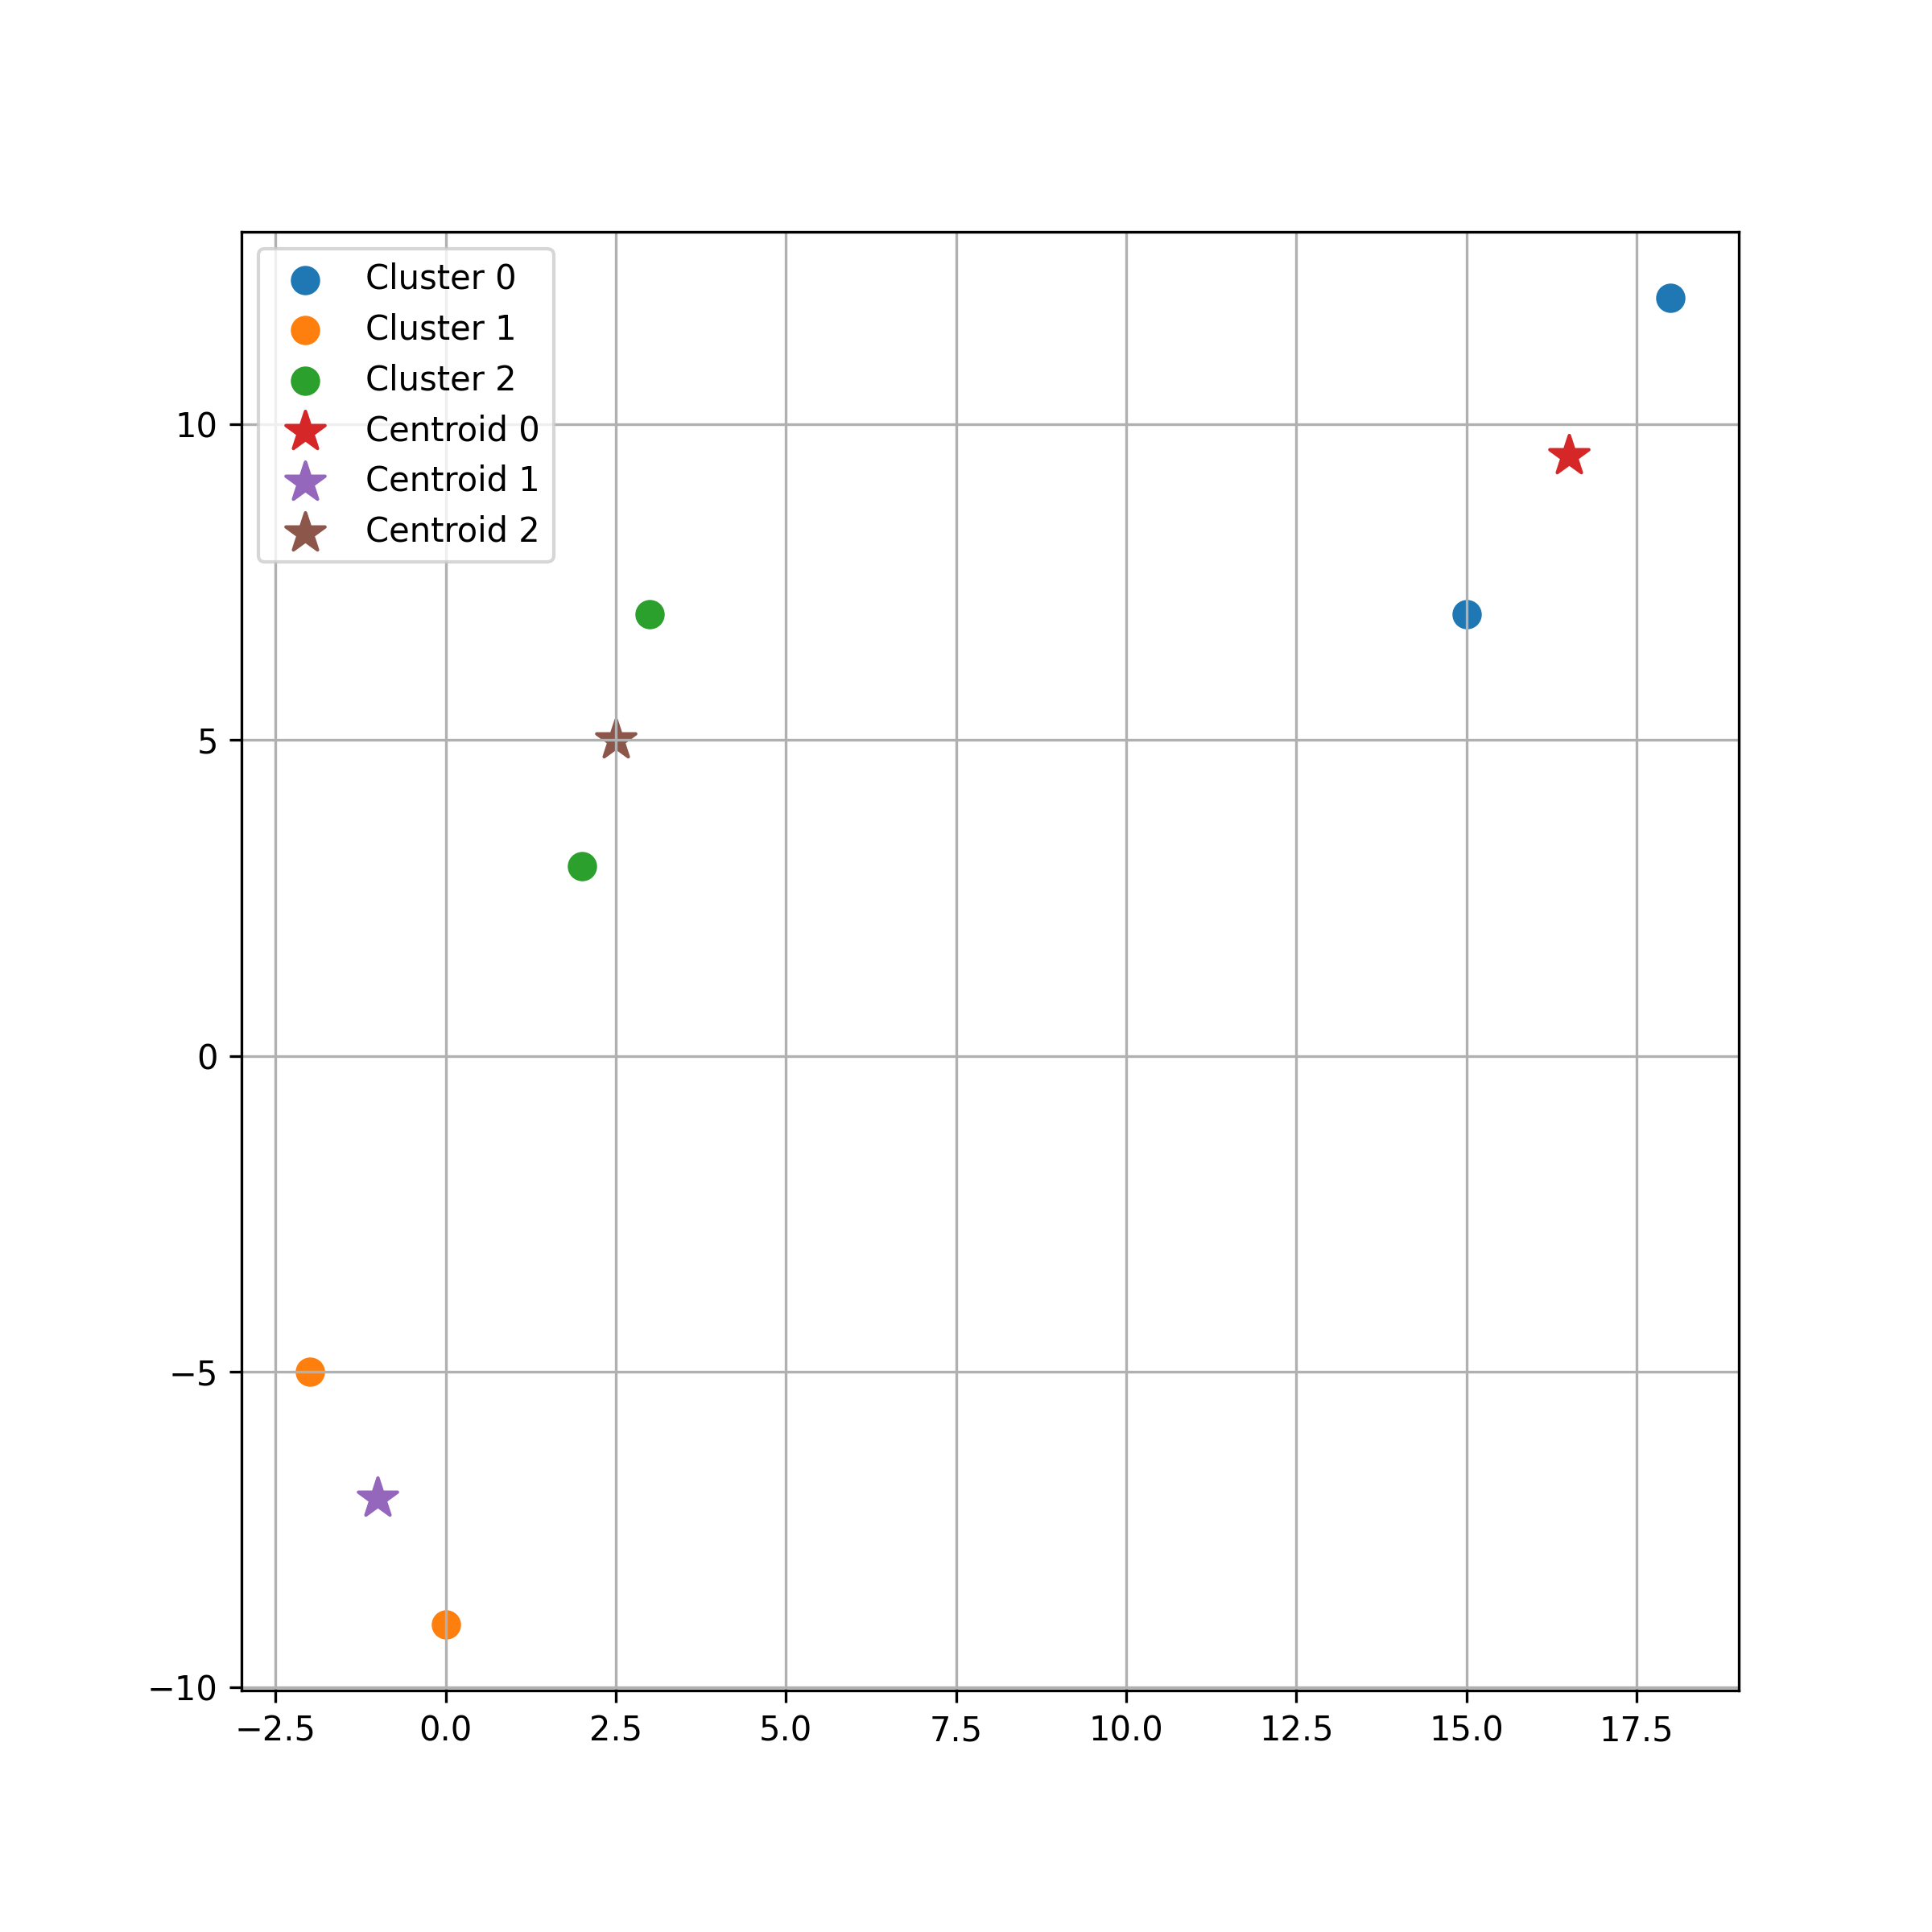
\includegraphics[width=0.7\textwidth]{p01.png}
\end{center}
\end{homeworkProblem}

\begin{homeworkProblem}
You are given the data set
\begin{equation*}
    \{ (3, 2)^{\top}, (-1, 0)^{\top}, (7, 1)^{\top} \}
\end{equation*}

\textit{Manually} compute the principle components of this data set by solving the associated eigenvalue problem.

Recalling Theorem 9.2 for finding the solution of the optimization problem:\\

Let the setting of Theorem 9.1 be given. The solution $\hat{\mathcal{V}}_{d}$ of the optimization problem is the matrix composed of the eigenvectors for the $d$ largest eigenvalues of the matrix
\begin{equation*}
    A = \mathcal{X}^{T}\mathcal{X}
\end{equation*}
where $\mathcal{X} \in \mathbb{R}^{N \times D}$ is the matrix created from the data as $\mathcal{X} = (\boldsymbol x_{1} | \ldots | \boldsymbol x_{N})^{\top}$.

Based on Theorem 9.1, the data needs to be centered. The mean of the given data set is $(3, 1)^{\top}$. The centered data set is then:
\begin{equation*}
    \{ (0, 1)^{\top}, (-4, -1)^{\top}, (4, 0)^{\top} \}
\end{equation*}

Calculating $A$ by performing the matrix multiplication of the transpose of the data set and the data set itself:
\begin{equation*}
    A = \begin{pmatrix} 0 & -4 & 4 \\ 1 & -1 & 0 \end{pmatrix} \begin{pmatrix} 0 & 1 \\ -4 & -1 \\ 4 & 0 \end{pmatrix} = \begin{pmatrix} 32 & 4 \\ 4 & 2 \end{pmatrix}
\end{equation*}

Finding the eigenvalues:
\begin{equation*}
    \text{det}(A - \lambda I) = \begin{vmatrix} 32 - \lambda & 4 \\ 4 & 2 - \lambda \end{vmatrix} = \lambda^{2} - 34 \lambda + 48 = (\lambda + \sqrt{241} - 17)(\lambda - \sqrt{241} + 17) = 0
\end{equation*}
The eigenvalues correspond to the solutions to the equation above. The eigenvalues are: $\lambda_{1} = -\sqrt{241} + 17 \approx 1.4758253$, $\lambda_{2} = \sqrt{241} + 17 \approx 32.5241747$

The eigenvectors corresponding to the eigenvalues are the principle components.

For $\lambda_{1} = -\sqrt{241} + 17$:
\begin{equation*}
    (A - \lambda_{1} I) \cdot \boldsymbol v = \begin{pmatrix} \sqrt{241} + 15 & 4 \\ 4 & \sqrt{241} - 15 \end{pmatrix} \cdot \boldsymbol v = 0
\end{equation*}

The solution set is represented by the eigenvector: $\begin{pmatrix} \frac{-\sqrt{241} + 15}{4} \\ 1 \end{pmatrix}$

For $\lambda_{2} = \sqrt{241} + 17$:
\begin{equation*}
    (A - \lambda_{2} I) \cdot \boldsymbol v = \begin{pmatrix} -\sqrt{241} + 15 & 4 \\ 4 & -\sqrt{241} - 15 \end{pmatrix} \cdot \boldsymbol v = 0
\end{equation*}

The solution set is represented by the eigenvector: $\begin{pmatrix} \frac{\sqrt{241} + 15}{4} \\ 1 \end{pmatrix}$

\end{homeworkProblem}

\begin{homeworkProblem}
A well-known application of principle component analysis is lossy data compression. In this application, you are given a large data set $\{ \mathbf{x} \}_{i = 1}^{N}$ with $\mathbf{x}_{i} \in \mathbb{R}^{D}$ and reduce it to a data set $\{ \bar{\mathbf{x}} \}_{i = 1}^{N}$ with $\bar{\mathbf{x}}_{i} \in \mathbb{R}^{d}$ where $d < D$, while storing a matrix that allows to reconstruct an approximation to the $\mathbf{x}_{i}$ from the vectors $\bar{\mathbf{x}}_{i}$.

Develop and give a compression and a decompression algorithm which carry out the above described data compression and decompression tasks by using principle component analysis. You can either try to develop the idea by yourself or do a research in the internet. In the latter case, please quote the source from which you took the information.

The followings are the algorithms to compress and decompress a set of data $\{ \mathbf{x} \}_{i = 1}^{N}$:\\


\textbf{Input:} input data $\{ \mathbf{x} \}_{i = 1}^{N}$, nr\_components\\
\textbf{Output:} compressed data  $\{ \bar{\mathbf{x}}_{i} \}_{i = 1}^{N}$
\begin{enumerate}
    \begin{enumerate}[a)]
        \item $Mean \gets mean(data)$
        \item $Zero\_Centered \leftarrow data - Mean x$
        \item $Cov\_Matrix \leftarrow (Zero\_Centered^{T} \cdot Zero\_Centered) / (length(data) - 1)$
        \item $eig\_values, eig\_vectors \leftarrow eig(Cov\_Matrix)$
        \item $selected\_components \leftarrow eig\_vectors[:, :nr\_components]$
        \item $compressed\_data \leftarrow selected\_components^{T} \cdot data^{T}$
        \item return $compressed\_data^{T}$
    \end{enumerate}

\end{enumerate}


\textbf{Input:} compressed data  $\{ \bar{\mathbf{x}}_{i} \}_{i = 1}^{N}$\\
\textbf{Output:} original data  $\{ {\mathbf{x}}_{i} \}_{i = 1}^{N}$
\begin{enumerate}
    \begin{enumerate}[a)]
        \item $decompressed\_data \gets compressed\_data \cdot selected\_components^{T}$
        \item return $decompressed\_data$
    \end{enumerate}

\end{enumerate}


\end{homeworkProblem}


\begin{programmingProblem}
In this task, you are supposed to apply your just developed data compression algorithm to the MNIST data set. To this end, consult again Example 9.4, which provides access to the hand-written digits for the value 8 in MNIST. Compress the images of these digits to a dimensionality of $d = 784, 512, 256, 128, 64, 32$, decompress them again, and plot the decompressed digits.

The implementation of the above algorithms can be found in the file \texttt{programming\_exercises.ipynb}.
\end{programmingProblem}
\end{document}